% !TEX program = xelatex
% Отчёт о лабораторной работе № 1 «Анализ и синтез комбинационных узлов ЭВМ. Дешифратор»
% Компиляция: xelatex report.tex (дважды — для содержания и ссылок)
% Рядом с файлом должны лежать рисунки fig3_dc38.png, fig5_id4.png, fig6_id4_3x8.png
\documentclass[14pt,a4paper]{extarticle}

% ---------- Шрифты и язык ----------
\usepackage{fontspec}
\IfFontExistsTF{Times New Roman}
  {\setmainfont{Times New Roman}}
  {\setmainfont{Liberation Serif}}
\IfFontExistsTF{Courier New}
  {\setmonofont{Courier New}}
  {\setmonofont{Liberation Mono}}
% Язык: babel (совместим со старыми и новыми версиями L3; polyglossia v2.8 требует свежего l3kernel)
\usepackage[english]{babel}
\babelprovide[import, main]{russian}
\usepackage{unicode-math}
\setmathfont{latinmodern-math.otf}
\IfFontExistsTF{Times New Roman}
  {\setmathfont[range={up/{latin,Latin,num}}]{Times New Roman}
   \setmathfont[range={it/{latin,Latin}}]{Times New Roman Italic}}
  {\setmathfont[range={up/{latin,Latin,num}}]{Liberation Serif}
   \setmathfont[range={it/{latin,Latin}}]{Liberation Serif Italic}}

% ---------- Поля и интервалы (ГОСТ 7.32-2001, п. 6.1.1) ----------
\usepackage[left=30mm,right=10mm,top=15mm,bottom=20mm,footskip=10mm]{geometry}
\usepackage{setspace}
\onehalfspacing
\setlength{\parindent}{1.25cm}
\usepackage{indentfirst}
\setlength{\parskip}{0pt}
\sloppy

% ---------- Заголовки ----------
\usepackage{titlesec}
\titleformat{\section}{\normalfont\bfseries}{\thesection}{0.6em}{}
\titleformat{\subsection}{\normalfont\bfseries}{\thesubsection}{0.6em}{}
\titlespacing*{\section}{\parindent}{18pt}{12pt}
\titlespacing*{\subsection}{\parindent}{12pt}{6pt}
\renewcommand{\thesection}{\arabic{section}}
\renewcommand{\thesubsection}{\thesection.\arabic{subsection}}

% Структурные элементы без номера: с новой страницы, по центру, прописными
\newcommand{\structsection}[1]{%
  \clearpage
  \phantomsection
  \addcontentsline{toc}{section}{#1}%
  \begin{center}\textbf{#1}\end{center}\vspace{6pt}}

% ---------- Содержание (без tocloft — совместимо со старым ядром LaTeX) ----------
\makeatletter
\renewcommand{\tableofcontents}{%
  {\centering\textbf{СОДЕРЖАНИЕ}\par}\vspace{12pt}%
  \@starttoc{toc}}
\renewcommand*{\l@section}{\@dottedtocline{1}{0pt}{1.5em}}
\renewcommand*{\l@subsection}{\@dottedtocline{2}{1.5em}{2.3em}}
\renewcommand{\@pnumwidth}{1.8em}
\makeatother

% ---------- Подписи рисунков и таблиц (ГОСТ 7.32-2001, пп. 6.5, 6.6) ----------
\usepackage{caption}
\DeclareCaptionLabelSeparator{gost}{~---~}
\captionsetup{labelsep=gost, font={normalsize}, skip=6pt}
\captionsetup[figure]{name=Рисунок, justification=centering}
\captionsetup[table]{name=Таблица, justification=raggedright, singlelinecheck=false, position=top}

% ---------- Таблицы, графика, формулы ----------
\usepackage{graphicx}
\usepackage{float}
\usepackage{array,tabularx,makecell,multirow}
\renewcommand{\arraystretch}{1.15}
\newcolumntype{C}{>{\centering\arraybackslash}X}
\newcolumntype{L}{>{\raggedright\arraybackslash}X}
\usepackage{amsmath}
\usepackage{tikz}
\usetikzlibrary{arrows.meta,positioning,calc}
\usepackage{enumitem}
\setlist{nosep, leftmargin=*, labelindent=\parindent, itemindent=0pt}
\newlist{gostlist}{enumerate}{1}
% Буквенная нумерация перечислений по ГОСТ 2.105-95 (без букв ё, з, й, о, ч, ъ, ы, ь)
\newcommand{\gostletter}[1]{\ifcase#1\or а\or б\or в\or г\or д\or е\or ж\or и\or к\or л\or м\or н\or п\fi}
\newcommand{\gostlettercnt}[1]{\gostletter{\value{#1}}}
\AddEnumerateCounter{\gostlettercnt}{\gostletter}{м}
\setlist[gostlist]{label=\gostlettercnt*), leftmargin=*, labelindent=\parindent, nosep}
\newlist{dashlist}{itemize}{1}
\setlist[dashlist]{label=--, leftmargin=*, labelindent=\parindent, nosep}

\usepackage{listings}
\lstset{basicstyle=\ttfamily\small, columns=fullflexible, frame=single}

\usepackage[hidelinks]{hyperref}

% ---------- Колонтитулы: номер страницы внизу по центру ----------
\pagestyle{plain}

% ---------- Данные для титульного листа (заполнить) ----------
\newcommand{\StudentName}{И.\,О.~Фамилия}
\newcommand{\StudentGroup}{5130201/50302}
\newcommand{\ReportDate}{23.09.2026}

% Обозначение инверсии
\newcommand{\inv}[1]{\overline{#1}}

\begin{document}
% ======================= ТИТУЛЬНЫЙ ЛИСТ =======================
\begin{titlepage}
\begin{singlespace}
\begin{center}
Министерство науки и высшего образования Российской Федерации\\[2pt]
Санкт-Петербургский политехнический университет Петра Великого\\[2pt]
Институт компьютерных наук и кибербезопасности\\[2pt]
Высшая школа технологий искусственного интеллекта

\vspace{5cm}

\textbf{ОТЧЁТ}\\[6pt]
\textbf{о лабораторной работе № 1}\\[12pt]
\textbf{«Анализ и синтез комбинационных узлов ЭВМ. Дешифратор»}\\[12pt]
по дисциплине «Основы архитектуры ЦВМ»
\end{center}

\vspace{4cm}

\noindent
\begin{tabular}{@{}p{7.2cm}p{3.6cm}l@{}}
Выполнил\\
студент гр. \StudentGroup & \underline{\hspace{3cm}} & Р.\,Ю.~Дужнов\\[22pt]
Проверил\\
доцент, к.\,т.\,н. & \underline{\hspace{3cm}} & Н.\,М.~Вербова\\
\end{tabular}

\vspace{1.2cm}
\noindent\hfill «\underline{\hspace{0.9cm}}» \underline{\hspace{3.2cm}} 2026 г.

\vfill
\begin{center}
Санкт-Петербург\\
2026
\end{center}
\end{singlespace}
\end{titlepage}
\setcounter{page}{2}

% ======================= СОДЕРЖАНИЕ =======================
\begin{singlespace}
\tableofcontents
\end{singlespace}

% ======================= ВВЕДЕНИЕ =======================
\structsection{ВВЕДЕНИЕ}

Объектом исследования являются комбинационные узлы ЭВМ типа «дешифратор» и «демультиплексор». Работа выполнена в соответствии с методическими указаниями~[1].

Цель работы~--- изучение принципов построения и функционирования дешифратора.

Для достижения цели решены следующие задачи:
\begin{gostlist}
\item синтезирована по заданной таблице истинности схема дешифратора трёхразрядного двоичного кода на элементах И, НЕ;
\item введена модель синтезированной схемы в среду схемотехнического моделирования и проверено её функционирование на всех входных наборах;
\item изучен принцип работы интегральной микросхемы (ИС) К155ИД4 (зарубежный аналог SN74155);
\item собрана схема исследования ИС К155ИД4 и исследована её работа в режимах двойного дешифратора 2 на 4 и демультиплексора 1 на 4;
\item разработана видоизменённая схема включения ИС К155ИД4, реализующая дешифратор 3 на 8, и проверена её работа.
\end{gostlist}

Моделирование выполнено в среде NI Multisim, являющейся развитием пакета Electronics Workbench, для которого составлены методические указания~[1].

% ======================= 1 =======================
\clearpage
\section{Теоретические сведения}

\subsection{Представление переключательных функций в СДНФ}

Переключательной функцией называется двоичная переменная $y$, значение которой однозначно определяется набором значений двоичных аргументов $x_{n-1}, \ldots, x_1, x_0$~[1]. Функция $n$ аргументов задаётся таблицей истинности, содержащей $2^n$ наборов.

Конституентой единицы (минтермом) называется функция $n$ переменных, равная единице только на одном наборе значений аргументов. Конституента единицы, соответствующая набору с номером $j$, записывается в виде
\begin{equation}
K_j = \tilde{x}_{n-1} \cdot \ldots \cdot \tilde{x}_1 \cdot \tilde{x}_0, \qquad
\tilde{x}_i =
\begin{cases}
x_i, & \text{если } a_i = 1,\\
\inv{x_i}, & \text{если } a_i = 0,
\end{cases}
\end{equation}
\noindent где $K_j$~--- конституента единицы набора с номером $j$;\\
$x_i$~--- $i$-й аргумент функции;\\
$a_i$~--- значение $i$-го разряда двоичной записи номера набора $j = \sum_{i=0}^{n-1} a_i \cdot 2^i$;\\
$n$~--- число аргументов.

Любая переключательная функция, не равная тождественно нулю, представляется в совершенной дизъюнктивной нормальной форме (СДНФ) как дизъюнкция конституент единицы тех наборов, на которых функция равна единице:
\begin{equation}
y = \bigvee_{j \in J_1} K_j,
\end{equation}
\noindent где $J_1$~--- множество номеров наборов, на которых $y = 1$.

Набор элементов И, ИЛИ, НЕ функционально полон, поэтому выражение~(2) непосредственно реализуется логической схемой. Перед построением схемы выражение упрощается с использованием приёмов склеивания, поглощения, вынесения и внесения за скобки~[1].

\subsection{Дешифратор и демультиплексор}

Дешифратором называется комбинационная схема, преобразующая поступающий на её входы код числа в управляющий сигнал, формируемый только на том выходе, номер которого соответствует коду на входах~[1]. Дешифратор, у которого число выходов равно числу всех возможных входных кодов, называется полным. Для полного дешифратора
\begin{equation}
N = 2^n,
\end{equation}
\noindent где $N$~--- число выходов;\\
$n$~--- разрядность входного кода.

Демультиплексором называется коммутатор, передающий сигнал с одного информационного входа в тот выходной канал, номер которого задан кодом на адресных входах~[1]. Структурно демультиплексор совпадает с дешифратором, дополненным информационным входом, по которому разрешается работа всех элементов И.

% ======================= 2 =======================
\section{Синтез дешифратора 3 на 8}

\subsection{Исходные данные}

Исходными данными для синтеза являются переключательные функции восьми выходов $y_0$--$y_7$ от трёх аргументов $x_2$, $x_1$, $x_0$, заданные таблицей истинности (таблица~\ref{tab:task}). Аргумент $x_2$ является старшим разрядом входного кода, $x_0$~--- младшим. В соответствии с формулой~(3) при $n = 3$ дешифратор имеет $N = 8$ выходов.

\begin{table}[H]
\caption{Таблица истинности дешифратора 3 на 8}
\label{tab:task}
\centering\small
\begin{tabularx}{\textwidth}{|c|C|C|C|C|C|C|C|C|C|C|C|}
\hline
№ набора & $x_2$ & $x_1$ & $x_0$ & $y_0$ & $y_1$ & $y_2$ & $y_3$ & $y_4$ & $y_5$ & $y_6$ & $y_7$ \\ \hline
0 & 0 & 0 & 0 & 1 & 0 & 0 & 0 & 0 & 0 & 0 & 0 \\ \hline
1 & 0 & 0 & 1 & 0 & 1 & 0 & 0 & 0 & 0 & 0 & 0 \\ \hline
2 & 0 & 1 & 0 & 0 & 0 & 1 & 0 & 0 & 0 & 0 & 0 \\ \hline
3 & 0 & 1 & 1 & 0 & 0 & 0 & 1 & 0 & 0 & 0 & 0 \\ \hline
4 & 1 & 0 & 0 & 0 & 0 & 0 & 0 & 1 & 0 & 0 & 0 \\ \hline
5 & 1 & 0 & 1 & 0 & 0 & 0 & 0 & 0 & 1 & 0 & 0 \\ \hline
6 & 1 & 1 & 0 & 0 & 0 & 0 & 0 & 0 & 0 & 1 & 0 \\ \hline
7 & 1 & 1 & 1 & 0 & 0 & 0 & 0 & 0 & 0 & 0 & 1 \\ \hline
\end{tabularx}
\end{table}

\subsection{Аналитические выражения выходных функций}

Каждая функция $y_k$ равна единице ровно на одном наборе~--- наборе с номером $k$ (таблица~\ref{tab:task}). Следовательно, множество $J_1$ в формуле~(2) для каждой функции содержит единственный элемент, и СДНФ функции $y_k$ совпадает с конституентой единицы $K_k$, записанной по формуле~(1):
\begin{align}
y_0 &= \inv{x_2}\cdot\inv{x_1}\cdot\inv{x_0}, & y_4 &= x_2\cdot\inv{x_1}\cdot\inv{x_0}, \\
y_1 &= \inv{x_2}\cdot\inv{x_1}\cdot x_0,      & y_5 &= x_2\cdot\inv{x_1}\cdot x_0, \\
y_2 &= \inv{x_2}\cdot x_1\cdot\inv{x_0},      & y_6 &= x_2\cdot x_1\cdot\inv{x_0}, \\
y_3 &= \inv{x_2}\cdot x_1\cdot x_0,           & y_7 &= x_2\cdot x_1\cdot x_0,
\end{align}
\noindent где $y_0$--$y_7$~--- выходные функции дешифратора;\\
$x_2$, $x_1$, $x_0$~--- разряды входного кода.

\subsection{Минимизация}

Приём склеивания $A x + A \inv{x} = A$ применим только к паре конституент одной функции, различающихся значением одной переменной. Каждая из функций~(4)--(7) содержит единственную конституенту, поэтому пары для склеивания отсутствуют. На карте Карно любой из функций $y_k$ единица занимает одну изолированную клетку, которой соответствует контур из одной клетки и произведение всех $n = 3$ переменных. Приёмы поглощения, вынесения и внесения за скобки к одночленному выражению также неприменимы.

Таким образом, выражения~(4)--(7) являются минимальными, и этап упрощения не изменяет состава схемы. Этот результат следует из самого назначения полного дешифратора: его выходные функции взаимно исключающи, и каждая из них выделяет ровно один входной код.

\subsection{Структура схемы}

Из выражений~(4)--(7) определяется состав схемы:
\begin{dashlist}
\item три элемента НЕ (DD1--DD3) для получения инверсных значений $\inv{x_2}$, $\inv{x_1}$, $\inv{x_0}$;
\item восемь трёхвходовых элементов И (DD4--DD11) для реализации конъюнкций $y_0$--$y_7$.
\end{dashlist}

Входы и выходы элементов НЕ образуют шесть шин: три прямые ($x_2$, $x_1$, $x_0$) и три инверсные ($\inv{x_2}$, $\inv{x_1}$, $\inv{x_0}$). Вход элемента И, формирующего выход $y_k$, подключается к прямой шине $x_i$, если $i$-й разряд двоичной записи числа $k$ равен единице, и к инверсной шине $\inv{x_i}$, если этот разряд равен нулю. Полученная таблица соединений приведена в таблице~\ref{tab:conn}.

\begin{table}[H]
\caption{Подключение входов элементов И к шинам}
\label{tab:conn}
\centering\small
\begin{tabularx}{\textwidth}{|C|C|C|C|C|}
\hline
Элемент & Выход & Вход 1 & Вход 2 & Вход 3 \\ \hline
DD4  & $y_0$ & $\inv{x_2}$ & $\inv{x_1}$ & $\inv{x_0}$ \\ \hline
DD5  & $y_1$ & $\inv{x_2}$ & $\inv{x_1}$ & $x_0$ \\ \hline
DD6  & $y_2$ & $\inv{x_2}$ & $x_1$ & $\inv{x_0}$ \\ \hline
DD7  & $y_3$ & $\inv{x_2}$ & $x_1$ & $x_0$ \\ \hline
DD8  & $y_4$ & $x_2$ & $\inv{x_1}$ & $\inv{x_0}$ \\ \hline
DD9  & $y_5$ & $x_2$ & $\inv{x_1}$ & $x_0$ \\ \hline
DD10 & $y_6$ & $x_2$ & $x_1$ & $\inv{x_0}$ \\ \hline
DD11 & $y_7$ & $x_2$ & $x_1$ & $x_0$ \\ \hline
\end{tabularx}
\end{table}

Каждая прямая и каждая инверсная шина нагружена на четыре входа элементов И, что следует из равенства числа нулей и единиц в каждом разряде кодов 0--7.

Сложность схемы оценена по Квайну~--- суммарным числом входов логических элементов:
\begin{equation}
Q = n + n \cdot 2^n = 3 + 3 \cdot 8 = 27,
\end{equation}
\noindent где $Q$~--- цена схемы по Квайну;\\
$n$~--- число входов дешифратора (слагаемое $n$ соответствует входам элементов НЕ, слагаемое $n \cdot 2^n$~--- входам элементов И).

Из формулы~(8) следует, что при одноступенчатой реализации затраты оборудования растут пропорционально $n \cdot 2^n$: при $n = 4$ цена составляет уже 68, а число входов каждого элемента И равно разрядности кода. Поэтому дешифраторы большой разрядности строятся каскадированием дешифраторов меньшей разрядности, что рассмотрено в разделе~5.

Функциональная схема стенда для проверки дешифратора составлена по образцу методических указаний~[1] и приведена на рисунке~\ref{fig:func}. Схема электрическая принципиальная синтезированного дешифратора, построенная по выражениям~(4)--(7) и таблице~\ref{tab:conn}, приведена на рисунке~\ref{fig:logic}.

\begin{figure}[H]
\centering
\begin{tikzpicture}[font=\small, box/.style={draw, minimum height=3.2cm, align=center, text width=3.4cm}]
\node[box] (sw) at (0,0) {Блок\\переключателей};
\node[box] (dc) at (6.2,0) {Схема\\электрическая\\принципиальная\\дешифратора};
\node[box] (ind) at (12.4,0) {Блок\\индикации};
\foreach \i/\y in {0/0.8,1/0,2/-0.8} {
  \draw ($(sw.east)+(0,\y)$) -- node[above]{$x_{\i}$} ($(dc.west)+(0,\y)$);
}
\foreach \i/\y in {0/1.0,1/0.35} {
  \draw ($(dc.east)+(0,\y)$) -- node[above]{$y_{\i}$} ($(ind.west)+(0,\y)$);
}
\node at ($(dc.east)!0.5!(ind.west)+(0,-0.3)$) {$\vdots$};
\draw ($(dc.east)+(0,-1.1)$) -- node[above]{$y_{7}$} ($(ind.west)+(0,-1.1)$);
\end{tikzpicture}
\caption{Функциональная схема стенда для проверки дешифратора}
\label{fig:func}
\end{figure}

\begin{figure}[H]
\centering
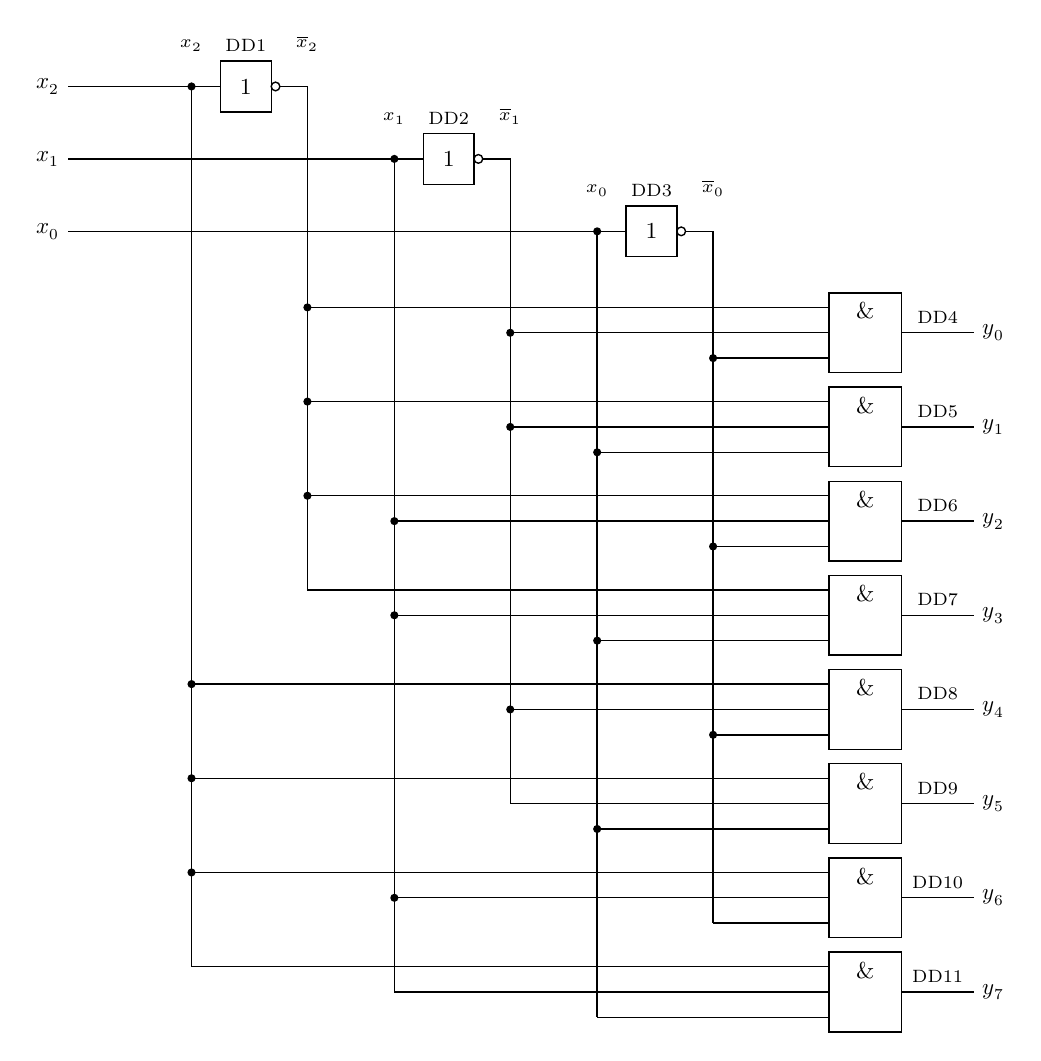
\begin{tikzpicture}[scale=0.92, transform shape, line width=0.5pt, font=\small]
\draw (-0.3,3.4) node[left]{$x_2$} -- (1.7999999999999998,3.4);
\fill (1.4,3.4) circle (1.6pt);
\draw (1.4,3.4) -- (1.4,-8.75);
\draw (1.7999999999999998,3.05) rectangle (2.5,3.75); \node at (2.15,3.4) {1};
\draw (2.5599999999999996,3.4) circle (0.06);
\draw (2.62,3.4) -- (3.0,3.4) -- (3.0,-3.55);
\node[font=\scriptsize,above] at (2.15,3.75) {DD1};
\node[font=\scriptsize,above] at (1.4,3.75) {$x_2$};
\node[font=\scriptsize,above] at (3.0,3.75) {$\overline{x}_2$};
\draw (-0.3,2.4) node[left]{$x_1$} -- (4.6000000000000005,2.4);
\fill (4.2,2.4) circle (1.6pt);
\draw (4.2,2.4) -- (4.2,-9.1);
\draw (4.6000000000000005,2.05) rectangle (5.300000000000001,2.75); \node at (4.95,2.4) {1};
\draw (5.36,2.4) circle (0.06);
\draw (5.42,2.4) -- (5.800000000000001,2.4) -- (5.800000000000001,-6.5);
\node[font=\scriptsize,above] at (4.95,2.75) {DD2};
\node[font=\scriptsize,above] at (4.2,2.75) {$x_1$};
\node[font=\scriptsize,above] at (5.800000000000001,2.75) {$\overline{x}_1$};
\draw (-0.3,1.4) node[left]{$x_0$} -- (7.4,1.4);
\fill (7.0,1.4) circle (1.6pt);
\draw (7.0,1.4) -- (7.0,-9.45);
\draw (7.4,1.0499999999999998) rectangle (8.1,1.75); \node at (7.75,1.4) {1};
\draw (8.16,1.4) circle (0.06);
\draw (8.22,1.4) -- (8.6,1.4) -- (8.6,-8.15);
\node[font=\scriptsize,above] at (7.75,1.75) {DD3};
\node[font=\scriptsize,above] at (7.0,1.75) {$x_0$};
\node[font=\scriptsize,above] at (8.6,1.75) {$\overline{x}_0$};
\draw (3.0,0.35) -- (10.2,0.35);
\fill (3.0,0.35) circle (1.6pt);
\draw (5.800000000000001,0.0) -- (10.2,0.0);
\fill (5.800000000000001,0.0) circle (1.6pt);
\draw (8.6,-0.35) -- (10.2,-0.35);
\fill (8.6,-0.35) circle (1.6pt);
\draw (3.0,-0.95) -- (10.2,-0.95);
\fill (3.0,-0.95) circle (1.6pt);
\draw (5.800000000000001,-1.3) -- (10.2,-1.3);
\fill (5.800000000000001,-1.3) circle (1.6pt);
\draw (7.0,-1.65) -- (10.2,-1.65);
\fill (7.0,-1.65) circle (1.6pt);
\draw (3.0,-2.25) -- (10.2,-2.25);
\fill (3.0,-2.25) circle (1.6pt);
\draw (4.2,-2.6) -- (10.2,-2.6);
\fill (4.2,-2.6) circle (1.6pt);
\draw (8.6,-2.95) -- (10.2,-2.95);
\fill (8.6,-2.95) circle (1.6pt);
\draw (3.0,-3.55) -- (10.2,-3.55);
\draw (4.2,-3.9) -- (10.2,-3.9);
\fill (4.2,-3.9) circle (1.6pt);
\draw (7.0,-4.25) -- (10.2,-4.25);
\fill (7.0,-4.25) circle (1.6pt);
\draw (1.4,-4.85) -- (10.2,-4.85);
\fill (1.4,-4.85) circle (1.6pt);
\draw (5.800000000000001,-5.2) -- (10.2,-5.2);
\fill (5.800000000000001,-5.2) circle (1.6pt);
\draw (8.6,-5.55) -- (10.2,-5.55);
\fill (8.6,-5.55) circle (1.6pt);
\draw (1.4,-6.15) -- (10.2,-6.15);
\fill (1.4,-6.15) circle (1.6pt);
\draw (5.800000000000001,-6.5) -- (10.2,-6.5);
\draw (7.0,-6.85) -- (10.2,-6.85);
\fill (7.0,-6.85) circle (1.6pt);
\draw (1.4,-7.45) -- (10.2,-7.45);
\fill (1.4,-7.45) circle (1.6pt);
\draw (4.2,-7.8) -- (10.2,-7.8);
\fill (4.2,-7.8) circle (1.6pt);
\draw (8.6,-8.15) -- (10.2,-8.15);
\draw (1.4,-8.75) -- (10.2,-8.75);
\draw (4.2,-9.1) -- (10.2,-9.1);
\draw (7.0,-9.45) -- (10.2,-9.45);
\draw (10.2,-0.55) rectangle (11.2,0.55); \node at (10.7,0.3) {\&};
\draw (11.2,-0.0) -- (12.2,-0.0) node[right]{$y_0$};
\node[font=\scriptsize,above] at (11.7,-0.0) {DD4};
\draw (10.2,-1.85) rectangle (11.2,-0.75); \node at (10.7,-1.0) {\&};
\draw (11.2,-1.3) -- (12.2,-1.3) node[right]{$y_1$};
\node[font=\scriptsize,above] at (11.7,-1.3) {DD5};
\draw (10.2,-3.1500000000000004) rectangle (11.2,-2.05); \node at (10.7,-2.3000000000000003) {\&};
\draw (11.2,-2.6) -- (12.2,-2.6) node[right]{$y_2$};
\node[font=\scriptsize,above] at (11.7,-2.6) {DD6};
\draw (10.2,-4.45) rectangle (11.2,-3.3500000000000005); \node at (10.7,-3.6000000000000005) {\&};
\draw (11.2,-3.9000000000000004) -- (12.2,-3.9000000000000004) node[right]{$y_3$};
\node[font=\scriptsize,above] at (11.7,-3.9000000000000004) {DD7};
\draw (10.2,-5.75) rectangle (11.2,-4.65); \node at (10.7,-4.9) {\&};
\draw (11.2,-5.2) -- (12.2,-5.2) node[right]{$y_4$};
\node[font=\scriptsize,above] at (11.7,-5.2) {DD8};
\draw (10.2,-7.05) rectangle (11.2,-5.95); \node at (10.7,-6.2) {\&};
\draw (11.2,-6.5) -- (12.2,-6.5) node[right]{$y_5$};
\node[font=\scriptsize,above] at (11.7,-6.5) {DD9};
\draw (10.2,-8.350000000000001) rectangle (11.2,-7.250000000000001); \node at (10.7,-7.500000000000001) {\&};
\draw (11.2,-7.800000000000001) -- (12.2,-7.800000000000001) node[right]{$y_6$};
\node[font=\scriptsize,above] at (11.7,-7.800000000000001) {DD10};
\draw (10.2,-9.65) rectangle (11.2,-8.549999999999999); \node at (10.7,-8.799999999999999) {\&};
\draw (11.2,-9.1) -- (12.2,-9.1) node[right]{$y_7$};
\node[font=\scriptsize,above] at (11.7,-9.1) {DD11};
\end{tikzpicture}
\caption{Схема электрическая принципиальная дешифратора 3 на 8 на элементах НЕ и И}
\label{fig:logic}
\end{figure}

% ======================= 3 =======================
\section{Моделирование синтезированной схемы}

\subsection{Модель схемы}

Модель дешифратора введена в среде Multisim в соответствии со схемой на рисунке~\ref{fig:logic}. Применены следующие компоненты:
\begin{dashlist}
\item интерактивные цифровые константы X0, X1, X2~--- источники входных сигналов $x_0$, $x_1$, $x_2$; значение константы (0 или 1) изменяется во время моделирования без перестроения схемы;
\item идеальные цифровые элементы NOT (notX0, notX1, notX2)~--- формирователи инверсных шин;
\item идеальные цифровые элементы AND3 (Y0--Y7)~--- трёхвходовые элементы И, формирующие выходы $y_0$--$y_7$;
\item логические пробники с порогом срабатывания 2,5~В~--- индикаторы выходов; свечение пробника соответствует уровню логической единицы.
\end{dashlist}

Идеальные цифровые элементы выбраны вместо моделей конкретных серий ТТЛ, так как задачей данного этапа является проверка логической функции, а не электрических параметров; такие элементы не требуют подключения цепей питания и не вносят в модель задержек распространения и нагрузочных ограничений. Введённая схема приведена на рисунке~\ref{fig:dc38}.

\begin{figure}[H]
\centering
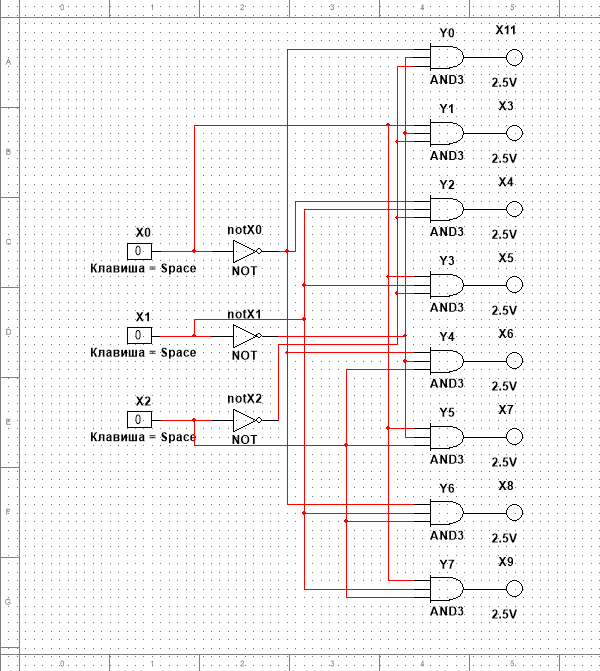
\includegraphics[width=0.85\textwidth]{fig3_dc38.png}
\caption{Модель дешифратора 3 на 8 на элементах NOT и AND3 в среде Multisim}
\label{fig:dc38}
\end{figure}

\subsection{Проверка функционирования}

Проверка выполнена методом полного перебора: на входы последовательно подавались все $2^3 = 8$ комбинаций входного кода, для каждой комбинации фиксировалось состояние восьми пробников. Результаты приведены в таблице~\ref{tab:sim38}.

\begin{table}[H]
\caption{Результаты моделирования синтезированного дешифратора}
\label{tab:sim38}
\centering\small
\begin{tabularx}{\textwidth}{|C|C|C|C|C|}
\hline
Входной код $x_2 x_1 x_0$ & Десятичный эквивалент & Ожидаемый активный выход & Светящийся пробник & Соответствие \\ \hline
000 & 0 & $y_0$ & Y0 & да \\ \hline
001 & 1 & $y_1$ & Y1 & да \\ \hline
010 & 2 & $y_2$ & Y2 & да \\ \hline
011 & 3 & $y_3$ & Y3 & да \\ \hline
100 & 4 & $y_4$ & Y4 & да \\ \hline
101 & 5 & $y_5$ & Y5 & да \\ \hline
110 & 6 & $y_6$ & Y6 & да \\ \hline
111 & 7 & $y_7$ & Y7 & да \\ \hline
\end{tabularx}
\end{table}

На каждой из восьми комбинаций светится ровно один пробник, номер которого равен десятичному эквиваленту входного кода; остальные семь пробников погашены. Результаты моделирования полностью совпадают с таблицей истинности (таблица~\ref{tab:task}), что подтверждает правильность синтеза. Активный уровень выходов синтезированной схемы~--- высокий (логическая единица).

% ======================= 4 =======================
\section{Исследование ИС К155ИД4 (SN74155)}

\subsection{Назначение и структура микросхемы}

ИС К155ИД4 содержит два дешифратора 2 на 4 (секции A и B) с общими адресными входами и инверсными выходами~[1]. Условное графическое обозначение микросхемы приведено на рисунке~\ref{fig:ugo}. Кружки на выводах выходов A0--A3 и B0--B3 обозначают инверсные выходы: выбранный выход переходит в состояние логического нуля, остальные выходы секции остаются в состоянии логической единицы.

\begin{figure}[H]
\centering
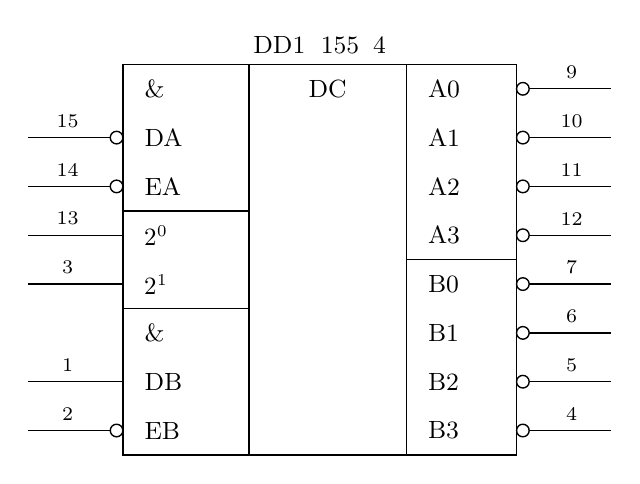
\begin{tikzpicture}[line width=0.5pt, font=\small, x=1cm, y=1cm]
\def\h{0.62}
% корпус
\draw (0,0) rectangle (5.0,-8*\h);
\draw (1.6,0) -- (1.6,-8*\h);
\draw (3.6,0) -- (3.6,-8*\h);
\node at (2.6,-0.5*\h) {DC};
% левое поле
\draw (0,-3*\h) -- (1.6,-3*\h);
\draw (0,-5*\h) -- (1.6,-5*\h);
\node[anchor=west] at (0.15,-0.5*\h) {\&};
\node[anchor=west] at (0.15,-5.5*\h) {\&};
\foreach \r/\lab/\pin/\invq in {1/DA/15/1, 2/EA/14/1, 3/$2^0$/13/0, 4/$2^1$/3/0, 6/DB/1/0, 7/EB/2/1} {
  \node[anchor=west] at (0.15,{-(\r+0.5)*\h}) {\lab};
  \ifnum\invq=1
    \draw (-0.08,{-(\r+0.5)*\h}) circle (0.08);
    \draw (-1.2,{-(\r+0.5)*\h}) -- (-0.16,{-(\r+0.5)*\h});
  \else
    \draw (-1.2,{-(\r+0.5)*\h}) -- (0,{-(\r+0.5)*\h});
  \fi
  \node[above, font=\scriptsize] at (-0.7,{-(\r+0.5)*\h}) {\pin};
}
% правое поле
\draw (3.6,-4*\h) -- (5.0,-4*\h);
\foreach \r/\lab/\pin in {0/A0/9, 1/A1/10, 2/A2/11, 3/A3/12, 4/B0/7, 5/B1/6, 6/B2/5, 7/B3/4} {
  \node[anchor=west] at (3.75,{-(\r+0.5)*\h}) {\lab};
  \draw (5.08,{-(\r+0.5)*\h}) circle (0.08);
  \draw (5.16,{-(\r+0.5)*\h}) -- (6.2,{-(\r+0.5)*\h});
  \node[above, font=\scriptsize] at (5.7,{-(\r+0.5)*\h}) {\pin};
}
\node[above] at (2.5,0) {DD1 К155ИД4};
\end{tikzpicture}
\caption{Условное графическое обозначение ИС К155ИД4}
\label{fig:ugo}
\end{figure}

Назначение выводов и их обозначения в модели 74155N среды Multisim приведены в таблице~\ref{tab:pins}. Имена выводов модели соответствуют обозначениям SN74155: секция B методических указаний соответствует секции 1 микросхемы, секция A~--- секции 2.

\begin{table}[H]
\caption{Назначение выводов ИС К155ИД4}
\label{tab:pins}
\centering\small
\begin{tabularx}{\textwidth}{|c|c|c|L|c|}
\hline
\makecell{Обозначение\\по [1]} & \makecell{Номер\\вывода} & \makecell{Имя вывода\\в модели 74155N} & \multicolumn{1}{c|}{Назначение} & \makecell{Активный\\уровень} \\ \hline
DA & 15 & \textasciitilde 2C & Информационный вход секции A & 0 \\ \hline
EA & 14 & \textasciitilde 2G & Стробирующий вход секции A & 0 \\ \hline
DB & 1 & 1C & Информационный вход секции B & 1 \\ \hline
EB & 2 & \textasciitilde 1G & Стробирующий вход секции B & 0 \\ \hline
$2^0$ & 13 & A & Адресный вход младшего разряда (вес 1), общий для секций & --- \\ \hline
$2^1$ & 3 & B & Адресный вход старшего разряда (вес 2), общий для секций & --- \\ \hline
A0--A3 & 9, 10, 11, 12 & \textasciitilde 2Y0--\textasciitilde 2Y3 & Выходы секции A & 0 \\ \hline
B0--B3 & 7, 6, 5, 4 & \textasciitilde 1Y0--\textasciitilde 1Y3 & Выходы секции B & 0 \\ \hline
\end{tabularx}
\end{table}

\subsection{Логические уравнения микросхемы}

Функционирование секций описывается следующими уравнениями, составленными по функциональной схеме SN74155:
\begin{equation}
A_k = \inv{\inv{DA} \cdot \inv{EA} \cdot m_k},
\end{equation}
\begin{equation}
B_k = \inv{DB \cdot \inv{EB} \cdot m_k},
\end{equation}
\begin{equation}
m_k = \tilde{a}_1 \cdot \tilde{a}_0, \qquad k = 2 a_1 + a_0,
\end{equation}
\noindent где $A_k$, $B_k$~--- уровни на выходах с номером $k$ секций A и B, $k = 0, \ldots, 3$;\\
$DA$, $DB$~--- уровни на информационных входах секций;\\
$EA$, $EB$~--- уровни на стробирующих входах секций;\\
$m_k$~--- конституента единицы адреса с номером $k$;\\
$a_1$, $a_0$~--- уровни на адресных входах $2^1$ и $2^0$;\\
$\tilde{a}_i$~--- переменная $a_i$ без инверсии при $i$-м разряде числа $k$, равном 1, и с инверсией при разряде, равном 0 (по аналогии с формулой~(1)).

Из уравнений~(9) и~(10) следуют условия разрешения работы секций: секция A работает при $DA = 0$ и $EA = 0$, секция B~--- при $DB = 1$ и $EB = 0$. Противоположная активность информационных входов DA и DB является конструктивной особенностью микросхемы, предназначенной для построения дешифратора 3 на 8 (раздел~5).

\subsection{Схема исследования}

Схема исследования собрана в среде Multisim по образцу схемы, приведённой в методических указаниях~[1, рис.~5], и показана на рисунке~\ref{fig:id4_1}. Уровни на входах DB, EB, $2^0$, $2^1$, DA, EA задаются шестью однополюсными переключателями на два направления (SPDT): в верхнем положении вход подключён к источнику питания VCC напряжением 5~В (логическая единица), в нижнем~--- к общему проводу (логический ноль). Состояние выходов A0--A3, B0--B3 отображается восемью логическими пробниками с порогом срабатывания 2,5~В.

Токоограничивающие резисторы и инверторы блока индикации, присутствующие в лабораторном стенде~[1], в модель не введены: логический пробник Multisim не потребляет тока от выхода и отображает непосредственно логический уровень. Вследствие инверсности выходов ИС при исправной работе разрешённой секции светятся три пробника из четырёх, а выбранный выход отмечается погашенным пробником.

\begin{figure}[H]
\centering
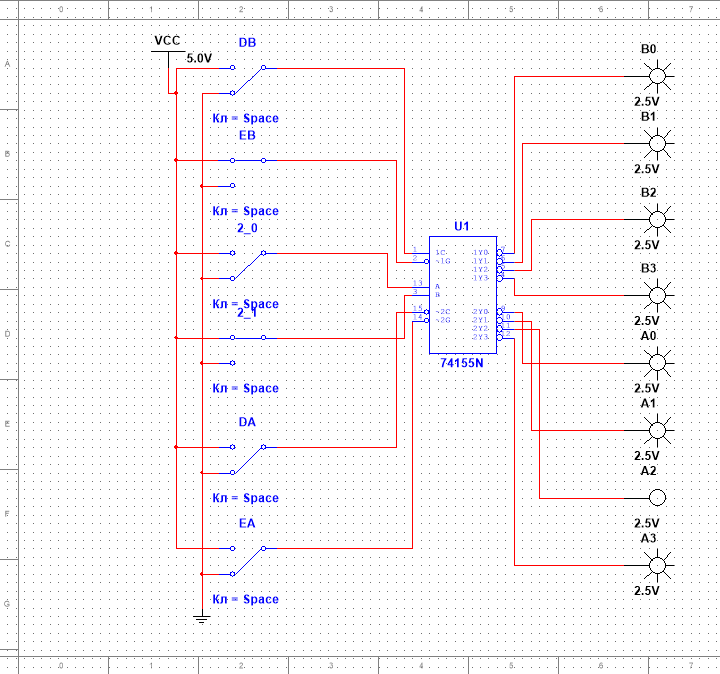
\includegraphics[width=0.9\textwidth]{fig5_id4.png}
\caption{Схема исследования ИС К155ИД4 в среде Multisim (DB~=~0, EB~=~1, адрес~10, DA~=~0, EA~=~0)}
\label{fig:id4_1}
\end{figure}

На рисунке~\ref{fig:id4_1} зафиксировано состояние, при котором секция A разрешена ($DA = 0$, $EA = 0$), код на адресных входах $2^1$, $2^0$ равен $10_2 = 2$, секция B заблокирована ($EB = 1$). Погашен только пробник A2, пробники A0, A1, A3 и B0--B3 светятся, что соответствует уравнениям~(9) и~(10).

\subsection{Режим двойного дешифратора 2 на 4}

Исследование выполнено раздельно для каждой секции. Для исключения взаимного влияния неисследуемая секция блокировалась единицей на стробирующем входе. Для каждой секции проверены все четыре адреса при разрешённой работе, а также действие стробирующего и информационного входов. Результаты приведены в таблицах~\ref{tab:secA} и~\ref{tab:secB}; в таблицах указаны логические уровни на выходах (0~--- пробник погашен, 1~--- пробник светится), символ «X» обозначает безразличное значение.

\begin{table}[H]
\caption{Результаты исследования секции A (EB = 1)}
\label{tab:secA}
\centering\small
\begin{tabularx}{\textwidth}{|c|c|c|c|c|c|c|c|L|}
\hline
EA & DA & $2^1$ & $2^0$ & A0 & A1 & A2 & A3 & \multicolumn{1}{c|}{Состояние секции} \\ \hline
1 & X & X & X & 1 & 1 & 1 & 1 & Заблокирована входом EA \\ \hline
0 & 1 & X & X & 1 & 1 & 1 & 1 & Заблокирована входом DA \\ \hline
0 & 0 & 0 & 0 & 0 & 1 & 1 & 1 & Выбран выход A0 \\ \hline
0 & 0 & 0 & 1 & 1 & 0 & 1 & 1 & Выбран выход A1 \\ \hline
0 & 0 & 1 & 0 & 1 & 1 & 0 & 1 & Выбран выход A2 \\ \hline
0 & 0 & 1 & 1 & 1 & 1 & 1 & 0 & Выбран выход A3 \\ \hline
\end{tabularx}
\end{table}

\begin{table}[H]
\caption{Результаты исследования секции B (EA = 1)}
\label{tab:secB}
\centering\small
\begin{tabularx}{\textwidth}{|c|c|c|c|c|c|c|c|L|}
\hline
EB & DB & $2^1$ & $2^0$ & B0 & B1 & B2 & B3 & \multicolumn{1}{c|}{Состояние секции} \\ \hline
1 & X & X & X & 1 & 1 & 1 & 1 & Заблокирована входом EB \\ \hline
0 & 0 & X & X & 1 & 1 & 1 & 1 & Заблокирована входом DB \\ \hline
0 & 1 & 0 & 0 & 0 & 1 & 1 & 1 & Выбран выход B0 \\ \hline
0 & 1 & 0 & 1 & 1 & 0 & 1 & 1 & Выбран выход B1 \\ \hline
0 & 1 & 1 & 0 & 1 & 1 & 0 & 1 & Выбран выход B2 \\ \hline
0 & 1 & 1 & 1 & 1 & 1 & 1 & 0 & Выбран выход B3 \\ \hline
\end{tabularx}
\end{table}

По результатам исследования установлено следующее:
\begin{gostlist}
\item номер активного выхода в каждой секции равен $2 a_1 + a_0$, где $a_1$, $a_0$~--- уровни на входах $2^1$ и $2^0$; адресные входы общие, поэтому при одновременно разрешённых секциях активны выходы с одинаковым номером в обеих группах;
\item единица на стробирующем входе EA (EB) переводит все выходы своей секции в неактивное состояние независимо от адреса и не влияет на другую секцию; это свойство используется для каскадирования микросхем и выборки одного корпуса из нескольких;
\item секция A блокируется единицей на входе DA, секция B~--- нулём на входе DB, что подтверждает противоположную активность информационных входов, следующую из уравнений~(9) и~(10).
\end{gostlist}

\subsection{Режим демультиплексора 1 на 4}

В режиме демультиплексора адресные входы задают номер канала, а на информационный вход подаётся передаваемый сигнал. Режим исследован на секции A: стробирующий вход EA установлен в ноль, секция B заблокирована входом EB, вход DA использован как информационный. При $EA = 0$ из уравнения~(9) следует:
\begin{equation}
A_k =
\begin{cases}
DA, & \text{если } m_k = 1,\\
1, & \text{если } m_k = 0,
\end{cases}
\end{equation}
\noindent где $A_k$~--- уровень на выходе с номером $k$ секции A;\\
$DA$~--- уровень на информационном входе;\\
$m_k$~--- конституента единицы адреса по формуле~(11).

Результаты исследования для двух адресов приведены в таблице~\ref{tab:demux}.

\begin{table}[H]
\caption{Результаты исследования режима демультиплексора 1 на 4 (EA = 0, EB = 1)}
\label{tab:demux}
\centering\small
\begin{tabularx}{\textwidth}{|C|C|C|C|C|C|C|}
\hline
$2^1$ & $2^0$ & DA & A0 & A1 & A2 & A3 \\ \hline
1 & 0 & 0 & 1 & 1 & 0 & 1 \\ \hline
1 & 0 & 1 & 1 & 1 & 1 & 1 \\ \hline
0 & 1 & 0 & 1 & 0 & 1 & 1 \\ \hline
0 & 1 & 1 & 1 & 1 & 1 & 1 \\ \hline
\end{tabularx}
\end{table}

Уровень на выходе, номер которого задан адресом, повторяет уровень на входе DA; остальные три выхода секции на изменение DA не реагируют и остаются в состоянии логической единицы. Следовательно, сигнал с одного входа передаётся в канал, выбранный адресом, что соответствует определению демультиплексора. Согласно уравнению~(9) сигнал через вход DA передаётся без инверсии; при использовании секции B и входа DB в соответствии с уравнением~(10) сигнал на выбранном выходе инвертируется ($B_k = \inv{DB}$ при $EB = 0$, $m_k = 1$).

Дешифратор и демультиплексор реализуются одной и той же структурой и различаются только назначением сигнала на информационном входе: постоянный разрешающий уровень соответствует режиму дешифратора, изменяющийся сигнал данных~--- режиму демультиплексора.

% ======================= 5 =======================
\section{Видоизменённая схема: дешифратор 3 на 8 на ИС К155ИД4}

\subsection{Принцип построения}

Для получения дешифратора 3 на 8 информационные входы DA (вывод 15) и DB (вывод 1) объединены в одну цепь, подключённую к переключателю «2\_2», стробирующие входы EA и EB установлены в ноль. Отдельные переключатели DA и DB исключены из схемы. При объединении входов $DA = DB = x_2$ уравнения~(9) и~(10) при $EA = EB = 0$ принимают вид:
\begin{equation}
y_k =
\begin{cases}
A_k = \inv{\inv{x_2} \cdot m_k}, & k = 0, \ldots, 3,\\
B_{k-4} = \inv{x_2 \cdot m_{k-4}}, & k = 4, \ldots, 7,
\end{cases}
\end{equation}
\noindent где $y_k$~--- уровень на выходе с номером $k$ дешифратора 3 на 8;\\
$x_2$~--- уровень на объединённом входе DA, DB;\\
$m_k$~--- конституента единицы адреса по формуле~(11).

Из уравнения~(13) следует, что при $x_2 = 0$ разрешена только секция A, при $x_2 = 1$~--- только секция B. Объединённый вход выбирает одну из двух групп выходов и приобретает смысл старшего разряда адреса с весом $2^2 = 4$; входы $2^1$ и $2^0$ выбирают выход внутри группы. Выходы A0--A3 становятся выходами $y_0$--$y_3$, выходы B0--B3~--- выходами $y_4$--$y_7$. Схема не требует дополнительных логических элементов, так как необходимая инверсия старшего разряда обеспечивается противоположной активностью входов DA и DB. Стробирующие входы EA и EB, объединённые в одну цепь, могут использоваться как общий вход разрешения дешифратора 3 на 8 либо как информационный вход демультиплексора 1 на 8.

Видоизменённая схема приведена на рисунке~\ref{fig:id4_2}. На рисунке зафиксировано состояние при коде $101_2 = 5$ на входах $2^2$, $2^1$, $2^0$: погашен только пробник B1, соответствующий выходу $y_5$.

\begin{figure}[H]
\centering
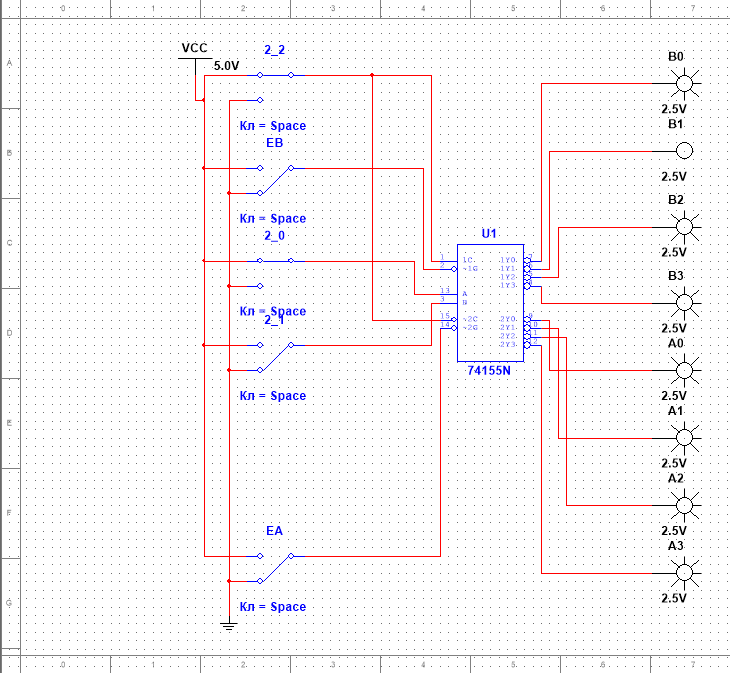
\includegraphics[width=0.92\textwidth]{fig6_id4_3x8.png}
\caption{Видоизменённая схема включения ИС К155ИД4~--- дешифратор 3 на 8 (входной код 101, EA~=~EB~=~0)}
\label{fig:id4_2}
\end{figure}

\subsection{Результаты исследования}

Работа схемы проверена на всех восьми комбинациях входного кода при $EA = EB = 0$. Результаты приведены в таблице~\ref{tab:dc38ic}.

\begin{table}[H]
\caption{Результаты исследования дешифратора 3 на 8 на ИС К155ИД4}
\label{tab:dc38ic}
\centering\small
\begin{tabularx}{\textwidth}{|C|C|C|C|C|}
\hline
Код на входах $2^2$, $2^1$, $2^0$ & Десятичный эквивалент & Разрешённая секция & Погашенный пробник & Выход дешифратора \\ \hline
000 & 0 & A & A0 & $y_0$ \\ \hline
001 & 1 & A & A1 & $y_1$ \\ \hline
010 & 2 & A & A2 & $y_2$ \\ \hline
011 & 3 & A & A3 & $y_3$ \\ \hline
100 & 4 & B & B0 & $y_4$ \\ \hline
101 & 5 & B & B1 & $y_5$ \\ \hline
110 & 6 & B & B2 & $y_6$ \\ \hline
111 & 7 & B & B3 & $y_7$ \\ \hline
\end{tabularx}
\end{table}

Соответствие входного кода и номера активного выхода полностью совпадает с таблицей истинности (таблица~\ref{tab:task}). Сравнение двух реализаций дешифратора 3 на 8 приведено в таблице~\ref{tab:compare}.

\begin{table}[H]
\caption{Сравнение реализаций дешифратора 3 на 8}
\label{tab:compare}
\centering\small
\begin{tabularx}{\textwidth}{|L|C|C|}
\hline
\multicolumn{1}{|c|}{Характеристика} & На элементах НЕ и И (раздел 2) & На ИС К155ИД4 (раздел 5) \\ \hline
Состав & 3 элемента НЕ, 8 элементов И & 1 корпус ИС \\ \hline
Активный уровень выходов & Высокий (1) & Низкий (0) \\ \hline
Вход разрешения & Отсутствует & EA, EB (активный уровень 0) \\ \hline
Возможность работы демультиплексором & Отсутствует & Имеется \\ \hline
Возможность каскадирования & Требует доработки схемы & Обеспечивается входами EA, EB \\ \hline
\end{tabularx}
\end{table}

Реализация на ИС отличается инверсной полярностью выходов и наличием входов разрешения. Для получения выходов с высоким активным уровнем к выходам ИС необходимо подключить инверторы.

% ======================= ЗАКЛЮЧЕНИЕ =======================
\structsection{ЗАКЛЮЧЕНИЕ}

В ходе выполнения лабораторной работы получены следующие результаты.

1. Синтезирован дешифратор 3 на 8 на элементах НЕ и И. Установлено, что выходные функции полного дешифратора в СДНФ являются одиночными конституентами единицы и не допускают упрощения, поэтому схема содержит три элемента НЕ и восемь трёхвходовых элементов И; цена схемы по Квайну составляет 27 и растёт пропорционально $n \cdot 2^n$.

2. Моделирование синтезированной схемы в среде Multisim на всех восьми входных наборах подтвердило соответствие схемы заданной таблице истинности: при каждом входном коде активен ровно один выход, номер которого равен десятичному эквиваленту кода.

3. Исследована ИС К155ИД4 в режиме двойного дешифратора 2 на 4. Подтверждено, что выходы микросхемы инверсные, адресные входы общие для обеих секций, стробирующие входы EA и EB блокируют каждую свою секцию независимо, а информационные входы имеют противоположную активность: секция A разрешается нулём на входе DA, секция B~--- единицей на входе DB.

4. Исследован режим демультиплексора 1 на 4: уровень на выходе, выбранном адресом, повторяет уровень на информационном входе DA, остальные выходы секции сохраняют неактивное состояние. Установлено, что дешифратор и демультиплексор имеют одинаковую структуру и различаются назначением сигнала на информационном входе.

5. Разработана видоизменённая схема включения ИС К155ИД4, реализующая дешифратор 3 на 8 без дополнительных элементов: объединённые входы DA и DB выполняют функцию старшего разряда адреса с весом 4. Результаты исследования полностью совпадают с таблицей истинности дешифратора 3 на 8 и отличаются от синтезированной схемы только низким активным уровнем выходов.

% ======================= ИСТОЧНИКИ =======================
\structsection{СПИСОК ИСПОЛЬЗОВАННЫХ ИСТОЧНИКОВ}

\begin{enumerate}[label=\arabic*, leftmargin=*, labelindent=\parindent, itemsep=0pt, align=left]
\item Вербова, Н.\,М. Изучение элементов и узлов ЭВМ : сборник описаний лабораторных работ по курсу «Архитектура ЭВМ» / Н.\,М.~Вербова.~--- Санкт-Петербург : СПбГПУ, 2011.~--- 58~с.
\end{enumerate}

\end{document}
